%更换squad。
\begin{table*}[ht!]
\centering
\scalebox{0.85}{
\begin{tabular}{cc|cc|cc|cc|cc}
\specialrule{0.1em}{0.2em}{0.2em}
\multicolumn{2}{c}{}&\multicolumn{2}{c}{CLINC150}&\multicolumn{2}{c}{StackOverflow}&\multicolumn{2}{c}{Banking}&\multicolumn{2}{c}{M-CID-EN}\\
&Methods & Accuracy & Macro-F1& Accuracy & Macro-F1& Accuracy & Macro-F1& Accuracy & Macro-F1\\
\specialrule{0.05em}{0.1em}{0.2em}
\multirow{6}{*}{25\%} 
                    &MSP&66.60 & 51.20 &33.94 &45.68  &48.15 &48.47 &52.05&43.14   \\
                    &DOC&64.43 & 44.60 &60.68 &60.51  &37.78 &46.35 &49.32&46.59  \\
                    &SEG&72.86 & 65.44 &47.00 &52.83  &51.11 &55.68 &44.51&50.14 \\
                    &LMCL& 68.57&62.42 &41.60 &48.21  &52.77 &56.73 &41.44&46.99  \\
                    &Softmax&76.50& 67.74 &46.17 &50.78  &57.88 & 58.32&41.95&45.46   \\
                    % &\bf {Ours} &\bf88.39 & \bf 74.49 &\bf79.88 & \bf 69.46 & \bf 82.15&\bf 67.96&\bf 78.38&\bf 69.83\\
                    &\bf {Ours} &\bf88.44 & \bf 80.73 &\bf68.74 & \bf 65.64 & \bf 74.11&\bf 69.93&\bf 87.08&\bf 79.67\\
\specialrule{0.05em}{0.1em}{0.2em}
\multirow{6}{*}{50\%} 
                    &MSP& 68.61& 51.20 &56.33 &62.92  &53.83 &65.33 &61.21&54.33  \\
                    &DOC& 62.46 & 70.01  &61.62 &68.97  &58.29 &57.30  &59.97&62.28 \\
                    &SEG& 77.05 & 79.42 & 68.50 & 74.18 &68.44 &76.48  &67.91&72.37 \\
                    &LMCL& 78.63& 80.42 &64.34 &71.80 & 63.59 &73.99 &63.42&69.04  \\
                    &Softmax&82.47&82.86 &65.96 &71.94  &67.44 &74.19 &64.72&69.35 \\
                    % &\bf {Ours}&\bf 85.44 &\bf 84.17 &\bf 78.17 &\bf 79.16 & \bf 74.91&\bf 77.34&\bf74.19&\bf75.12\\
                    &\bf {Ours}&\bf 88.33 &\bf 86.67 &\bf 75.08 &\bf 78.55 & \bf 72.69&\bf 79.21&\bf81.05&\bf79.73\\
\specialrule{0.05em}{0.1em}{0.2em}
\multirow{6}{*}{75\%} 
                    &MSP&73.41 &81.81  &76.73 & 77.63 &71.92 &80.77 &72.89&77.34  \\
                    &DOC&74.63 & 78.63 & 63.98 &62.07  &72.02 &78.04 &69.79&71.18  \\
                    &SEG&81.92 & 86.57  &80.83 &84.78  &78.87 &85.66 &75.73&79.97 \\
                    &LMCL& 84.59&88.21 &80.02 & 84.47  &78.66 &85.33 &77.11&80.96  \\
                    &Softmax& 86.26& 89.01 &77.41 &82.28  &78.20 &84.31 &76.99& 80.82 \\
                    % &\bf {Ours}&\bf85.08 & 86.30 &\bf81.08 & \bf85.11 &\bf79.32 &84.66&\bf77.14&79.53\\
                    &\bf {Ours}&\bf88.08 & \bf89.43 &\bf81.71 & \bf85.85 &\bf81.07 &\bf86.98&\bf80.24&\bf82.75\\
\specialrule{0.1em}{0.1em}{0.2em}
\end{tabular}
}
\caption{\label{mainresult1}
Overall accuracy and macro f1-score for unknown intent detection with different proportion of seen classes. For each setting, the best result is marked in bold. 
% For the 75\% setting, the top 2 results for each metric are marked in bold.
}
\end{table*}
In this section, we present the experimental results of our proposed method on the targeted task of unknown intent detection. Given a test set comprised of known and unknown intent classes, the primary goal of an unknown intent detection model is to assign correct intent labels to utterances in the test set. Notice that the unknown intent label $C_{oos}$ is also included as a special class for prediction. 
\begin{table}
\centering
% \setlength{\tabcolsep}{1.5pt}
% \footnotesize
\scalebox{0.76}{
\begin{tabular}{l|c|c|c|c}
\specialrule{0.05em}{0.1em}{0.2em}
Dataset & Vocab & Avg. Length & Samples & Classes\\
\specialrule{0.05em}{0.1em}{0.2em}
CLINC150&8,376&8.31&23,700&150\\
StackOverflow&17,182&9.18&20,000&20\\
Banking&5028&11.9&13,083&77\\
M-CID-EN&1,254&6.74&1,745&16\\
\specialrule{0.05em}{0.1em}{0.2em}
\end{tabular}
}
\caption{\label{table:datsets_stats}
Dataset statistics.
}
\end{table}

\begin{table*}[t]
\centering
\scalebox{0.90}{
\begin{tabular}{cc|cc|cc|cc|cc}
\specialrule{0.1em}{0.2em}{0.2em}
\multicolumn{2}{c}{}&\multicolumn{2}{c}{CLINC150}&\multicolumn{2}{c}{StackOverflow}&\multicolumn{2}{c}{Banking}&\multicolumn{2}{c}{M-CID-EN}\\
&Methods & Unknown & Known& Unknown & Known& Unknown & Known& Unknown & Known\\
\specialrule{0.05em}{0.1em}{0.2em}
\multirow{6}{*}{25\%} 
                    &MSP&73.20 &50.62  &22.59 &50.30  &49.98 &48.39 &56.27&37.86  \\
                    &DOC&71.08 &43.91  &66.11 &59.39  &31.41 &47.14  &53.08&44.92 \\
                    &SEG&79.90 &65.06  &46.17 &54.16  &53.22 &55.81 &42.73&51.99  \\
                    &LMCL&75.61 &62.01  &38.85 &50.15 &55.29 &56.81  &36.99&49.50 \\
                    &Softmax&83.04 &67.34  &45.52 &51.83  &62.52 &58.10 &35.39&46.22  \\
                    % &\bf {Ours} &\bf92.64 & \bf74.02 &\bf85.79 & \bf66.20 & \bf87.87&\bf67.00&\bf84.37&\bf66.20\\
                    &\bf {Ours} &\bf92.35 & \bf80.43 &\bf74.86 & \bf63.80 & \bf80.12&\bf69.39&\bf91.15&\bf76.80\\
\specialrule{0.05em}{0.1em}{0.2em}
\multirow{6}{*}{50\%} 
                    &MSP&57.78 &68.03  &35.18 &70.09  &29.31 &66.28 &58.55&53.80  \\
                    &DOC&57.62 &70.17  &47.96 &71.07  &49.88 &57.50  &47.22&64.16 \\
                    &SEG&78.02 &79.43  &60.89 &75.51 &60.42 &76.90&61.04 &73.80\\
                    &LMCL&79.89 &80.42  &53.12 &71.80  &50.30 &74.62  &51.11&71.29 \\
                    &Softmax&84.19 &82.84  &56.80 &73.45  &60.28 &74.56 &56.30&70.98  \\
                    % &\bf {Ours}&\bf87.48 &\bf84.12 &\bf77.68 &\bf79.31 & \bf73.91&\bf77.43&\bf73.50&\bf75.32\\
                    &\bf {Ours}&\bf90.30 &\bf86.54 &\bf71.88 &\bf79.22 & \bf67.26&\bf79.52&\bf82.44&\bf79.39\\
\specialrule{0.05em}{0.1em}{0.2em}
\multirow{6}{*}{75\%} 
                    &MSP&57.83 &82.02  &41.73 &80.03  &23.86 &81.75 &39.56&80.50  \\
                    &DOC&64.62 &78.76  &49.50&62.91  &39.47 &78.72 &49.41&72.99  \\
                    &SEG&76.12 &86.67  &62.30 &86.28  &54.43 &86.20 &51.51&82.34  \\
                    &LMCL&80.42 &88.28  &61.40 &84.47  &53.26 &85.89  &54.61&83.16 \\
                    &Softmax&83.12 &\bf89.61  &54.07&84.11  &56.90 &84.78 &58.73&82.66  \\
                    % &\bf {Ours}&\bf82.35 & 86.33 &\bf65.51 & \bf86.36 &\bf63.42 &85.03&\bf62.50&80.95\\
                    &\bf {Ours}&\bf86.28 &89.46 &\bf65.44 & \bf87.22 &\bf60.71 &\bf87.47&\bf69.00&\bf83.89\\
\specialrule{0.1em}{0.1em}{0.2em}
\end{tabular}
}
\caption{\label{mainresult2}
Macro f1-score of the known classes and f1-score of the unknown class with different proportion of seen classes. For each setting, the best result is marked in bold.
%For the 25\% and 50\% settings, the top 1 results for each metric are marked in bold. For the 75\% setting, the top 2 results for each metric are marked in bold.
}
\end{table*}
\subsection{Datasets and Baselines}
% \begin{figure*}[t]
%     \centering
%     \includegraphics[width=130mm]{number_ablation.png}
%     \caption{A study of the numbers of generated outliers.}
%     \label{fig:number_ablation}
% \end{figure*}

% We evaluate our proposed method on $4$ real task-oriented dialogueue datasets: CLINC150~\citep{larson2019evaluation}, StackOverflow~\citep{DBLP:conf/naacl/XuWTXZWH15}, Banking~\citep{DBLP:journals/corr/abs-2003-04807}, and M-CID-EN~\citep{arora2020cross}. The detailed statistics of datasets are summarized in Table~\ref{table:datsets_stats}. 
We evaluate our proposed method on four benchmark datasets as follows, three of which are newly released dialogue datasets designed for intent detection. The statistics of the datasets are summarized in Table~\ref{table:datsets_stats}. 

\textbf{CLINC150}~\citep{larson2019evaluation} is a dataset specially designed for out-of-scope intent detection, which consists of $150$ known intent classes from $10$ domains. The dataset includes $22,500$ in-scope queries and $1,200$ out-of-scope queries. For the in-scope ones, we follow the original splitting, i.e., $15,000$, $3,000$ and $4,500$ for training, validation, and testing respectively. For the out-of-scope ones, we group all of the $1,200$ queries into the test set. 

\textbf{StackOverflow}~\citep{DBLP:conf/naacl/XuWTXZWH15} consists of $20$ classes with $1,000$ examples in each class. We follow the original splitting, i.e., $12,000$ for training, $2,000$ for validation, and $6,000$ for test.

\textbf{Banking}~\citep{DBLP:journals/corr/abs-2003-04807} is a fine-grained intent detection dataset in the banking domain. It consists of $9,003$, $1,000$, and $3,080$ user queries in the training, validation, and test sets respectively.

% \textbf{M-CID}~\citep{arora2020cross} is a recently released multilingual intent detection dataset related to Covid-$19$, which consists of $1,745$ English utterances covering $16$ intent classes. We note the English subset of this dataset as M-CID-EN and use it in our experiments. The splitting of M-CID-EN is $1,258$ for training, $148$ for validation, and $339$ for test. 
\textbf{M-CID}~\citep{arora2020cross} is a recently released dataset related to Covid-$19$. We use the English subset of this dataset referred to as M-CID-EN in our experiments, which covers $16$ intent classes. The splitting of M-CID-EN is $1,258$ for training, $148$ for validation, and $339$ for test. 

We extensively compare our method with the following unknown intent detection methods.
\begin{itemize}
\item \textbf{Maximum Softmax Probability (MSP)}~\citep{DBLP:conf/iclr/HendrycksG17} employs the confidence score derived from the maximum softmax probability to predict the class of a sample. The idea under the hood is that the lower the confidence score is, the more likely the sample is of an unknown intent class.

\item \textbf{DOC}~\citep{DBLP:conf/emnlp/ShuXL17} considers to construct $m$ $1$-vs-rest sigmoid classifiers for $m$ seen classes respectively. It uses the maximum probability from these classifiers as the confidence score to conduct classification.

\item \textbf{SEG}~\citep{DBLP:conf/acl/YanFLLZWL20} models the intent distribution as a margin-constrained Gaussian mixture distribution and uses an additional outlier detector -- local outlier factor (LOF)~\citep{10.1145/335191.335388} to achieve unknown intent detection. 

\item \textbf{LMCL}~\citep{DBLP:conf/acl/LinX19} considers to learn discriminative embeddings with a large margin cosine loss. It also uses LOF as the outlier detection algorithm.

\item \textbf{Softmax}~\citep{DBLP:conf/acl/YanFLLZWL20} uses a softmax loss to learn discriminative features based on the training dataset, which also requires an additional outlier detector such as LOF for detecting the unknown intents. 
\end{itemize}

\begin{figure*}[t]
\begin{subfigure}{0.32\textwidth}
  \centering
  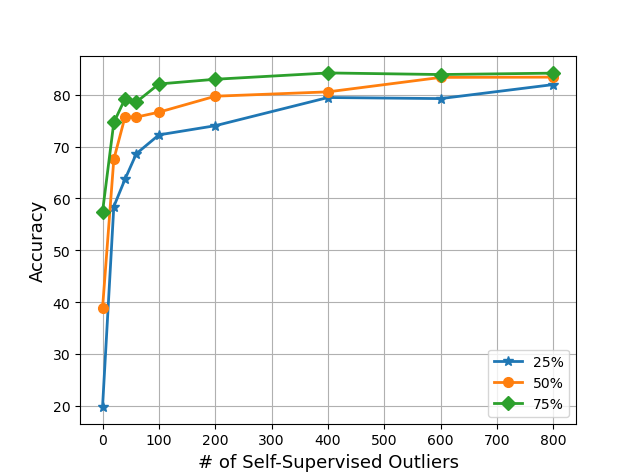
\includegraphics[width=1.1\linewidth]{acc_convex_new.png}
  \caption{ }
  \label{fig:convex_acc}
\end{subfigure}%
\begin{subfigure}{0.32\textwidth}
  \centering
  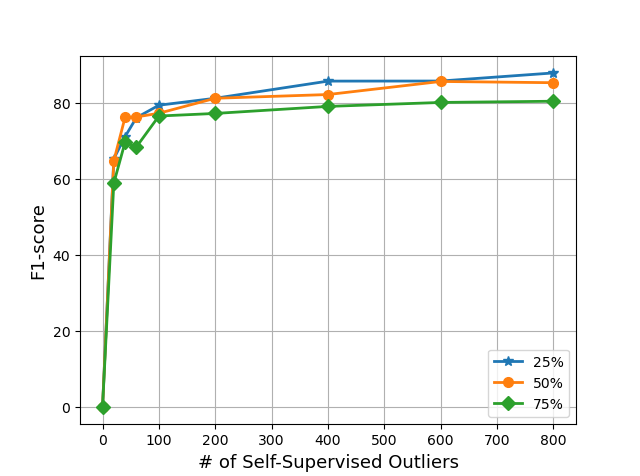
\includegraphics[width=1.1\linewidth]{F1_oos_convex_new.png}
  \caption{}
  \label{fig:convex_f1_unknown}
\end{subfigure}%
\begin{subfigure}{.32\textwidth}
  \centering
  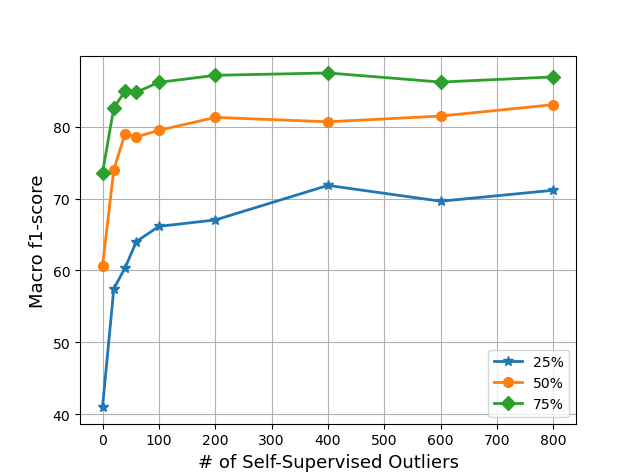
\includegraphics[width=1.1\linewidth]{macro_f1_convex_new.png}
  \caption{}
  \label{fig:convex_f1}
\end{subfigure}

\begin{subfigure}{.32\textwidth}
  \centering
  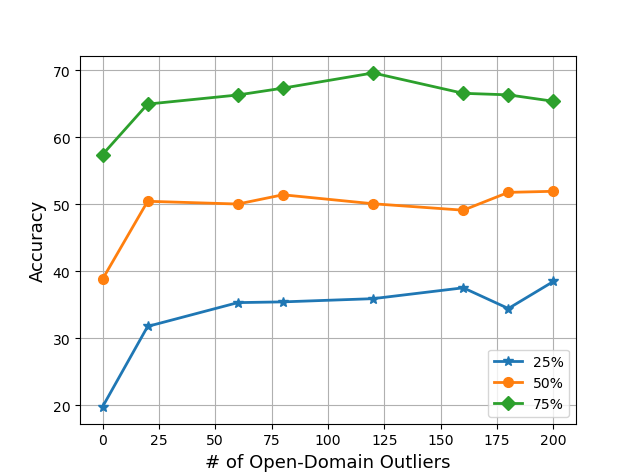
\includegraphics[width=1.1\linewidth]{acc_open_new.png}
  \caption{}
  \label{fig:open_domain_acc}
\end{subfigure}%
\begin{subfigure}{.32\textwidth}
  \centering
  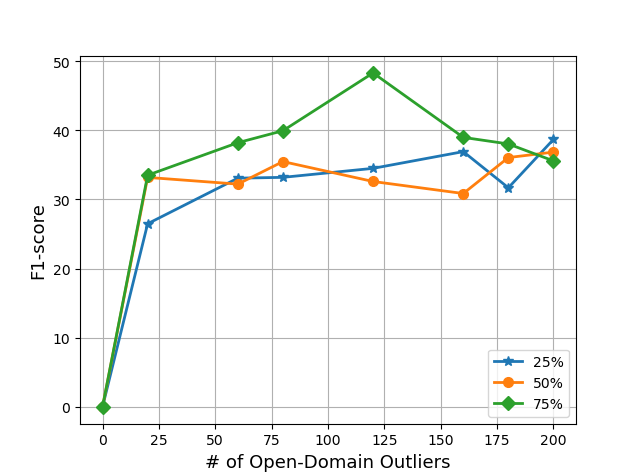
\includegraphics[width=1.1\linewidth]{f1_oos_open_new.png}
  \caption{}
  \label{fig:open_domain_f1_unknown}
\end{subfigure}%
\begin{subfigure}{.32\textwidth}
  \centering
  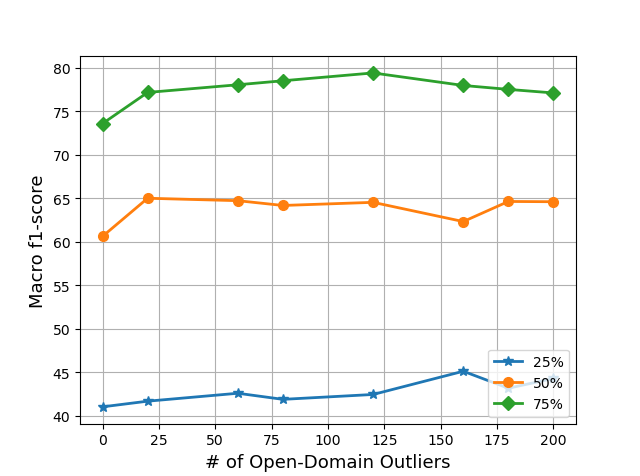
\includegraphics[width=1.1\linewidth]{macro_f1_open_new.png}
  \caption{}
  \label{fig:open_domain_f1}
\end{subfigure}
\caption{Effect of the number of pseudo outliers on CLINC150. %Sub-figures \ref{fig:convex_acc}, \ref{fig:convex_f1_unknown} and \ref{fig:convex_f1} 
(a), (b), and (c) display overall accuracy, f1-score on the unknown class and overall macro f1-score with varying number of self-supervised outliers respectively. 
%Sub-figures \ref{fig:open_domain_acc}, \ref{fig:open_domain_f1_unknown} and \ref{fig:open_domain_f1} 
(d), (e), and (f) display the corresponding results with varying number of open-domain outliers.}
% ,,
\label{fig:numbers}
\end{figure*}
\subsection{Experimental Setup and Evaluation Metrics}
To compare with existing methods, we follow the setting in LMCL~\citep{DBLP:conf/acl/LinX19}. Specifically, for each dataset, we randomly sample $75\%$, $50\%$, and $25\%$ of the intent classes from the training set as the known classes to conduct training, and we set aside the rest as the unknown classes for test. 
% Notice that for training and validation, we only use examples within the chosen known classes and our generated pseudo outliers.
Notice that for training and validation, we only use data within the chosen known classes and do not expose our model to any of test-time outliers. 
% Unless otherwise specified, in each training batch, we generate $\sim150$ and $800$ examples for the open-domain and self-supervised outliers respectively.
Unless otherwise specified, in each training batch, we keep the ratio of inliers, open-domain outliers and self-supervised outliers roughly as $1:1:4$. This setting is empirically chosen and affected by the memory limit of NVIDIA 2080TI GPU, which we use for conducting the experiments. The number of pseudo outliers can be adjusted according to different environments, and a larger number of self-supervised outliers typically takes more time to converge.
% and the number of labeled examples is selected according to the capacity of GPUs.

We use Pytorch~\citep{DBLP:conf/nips/PaszkeGMLBCKLGA19} as the backend to conduct the experiments. We use the pretrained BERT mdoel (\emph{bert-base-uncased}) provided by~\citet{wolf2019huggingface} as the encoder for utterances. We use the output vector of the special classification token [CLS] as the utterance embedding and fix its dimension as $768$ by default throughout all of our experiments. To ensure a fair comparison, all baselines and our model use the same encoder. 

%For the utterance representation of our model and baselines, our encoder is the pretrained BERT mdoel of \emph{bert-base-uncased} provided by~\citep{wolf2019huggingface}.

% In addition, we set the max length of input sentences for BERT as $30$, $45$, $55$, and $25$ for CLINC150, StackOverflow, Banking, and M-CID-EN respectively. 

For model optimization, we use AdamW provided by \citet{wolf2019huggingface} to fine-tune BERT and Adam proposed by \citet{DBLP:journals/corr/KingmaB14} to train the MLP clasisfier $\Phi(\cdot)$. We set the learning rate for BERT as $1e^{-5}$ as suggested by \citet{DBLP:conf/naacl/DevlinCLT19}. For the MLP clasisfier, the learning rate is fixed as $1e^{-4}$. Notice that the fine-tuning of BERT is conducted simultaneously with the training of the classifier $\Phi(\cdot)$ with the same cross-entropy loss. 
The MLP classifier $\Phi(\cdot)$ has a two-layer architecture with [$1024$, $1024$] as hidden units.
The temperature parameter $\tau$ is selected by cross-validation and set as $0.1$ in all experiments.

Following LMCL~\citep{DBLP:conf/acl/LinX19}, we use overall accuracy and macro f1-score as evaluation metrics. All results reported in this section are the average of $10$ runs with different random seeds, and each run is stopped until reaching a plateau on the validation set. For baselines, we follow their original training settings except using the aforementioned BERT as text encoder.  
\begin{figure}
  \centering
  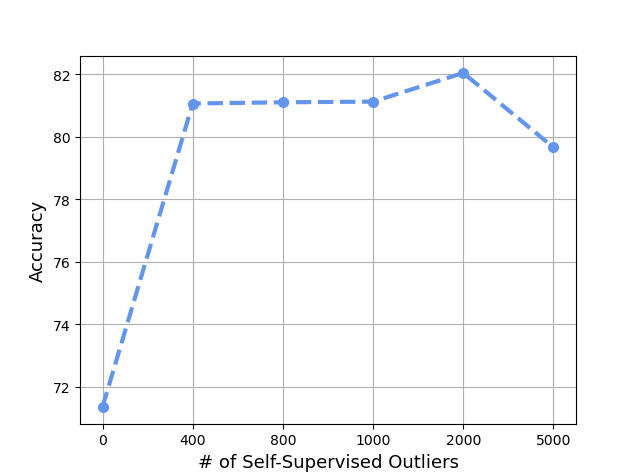
\includegraphics[width=1.\linewidth,height=0.19\textheight]{num_convex.png}
%\caption{Accuracy of the 75\% setting of Banking with different number of self-supervised outliers and the number of open-domain outliers fixed to $100$.}
\caption{Effect of the number of self-supervised outliers on overall intent detection accuracy under the 75\% setting of Banking.}
\label{fig:convex_num}
\end{figure}

\subsection{Result Analysis}
We present our main results in Table~\ref{mainresult1} and Table~\ref{mainresult2}. Specifically, Table~\ref{mainresult1} gives results in overall accuracy and macro f1-score for all classes including the outlier class, while Table~\ref{mainresult2} shows results in macro f1-score for the known classes and f1-score for the outlier class respectively. It can be seen that, on all benchmarks and in almost every setting, our model significantly outperforms the baselines. As shown in Table~\ref{mainresult2}, our method achieves favorable performance on both unknown and known intent classes simultaneously.

It is worth mentioning that the large improvements of our method in scenarios with small labeled training sets (25\% and 50\% settings) indicate its great potential in real-life applications, since a practical dialogue system often needs to deal with a larger proportion of outliers than inliers due to different user demographic, ignorance/unfamiliarity of/with the platform, and limited intent classes recognized by the system (especially at the early development stage). 
% As shown in Table~\ref{mainresult2}, our method can achieve favorable performance on both unknown and known intents simultaneously.
% because annotated training sets can be expensive and laborious to collect for dialogue systems and our goal is to recognize a finite group of known objects in myriad unknown objects~\citep{DBLP:journals/pami/ScheirerRSB13}.
%It is often the case that in real-life dialogue systems, training sets with labeled intents can be laborious to collect.The significant superiority of our method in scenarios with small labeled training sets demonstrates the great potential of our proposed method to be applied in real-life productions. Our method can achieve favorable performance not only for unknown intents but also for known intents.
% On the other hand, as shown in Table~\ref{mainresult1}, we can see that in the $75\%$ setting, our method is still among the best in accuracy, but slightly outperformed by some baselines in f1-score in several cases. However, as shown in Table~\ref{mainresult2}, when comparing with SEG, LMCL, and Softmax, it can be seen that their advantages are mainly in the known classes. However, our method can outperform them on the unknown classes. Take SEG and LMCL for example, they are all margin-based methods with different assumptions on intent distribution. As the proportion of known intents increases, they can better model known intents, which indicates they are more data-dependent. In contrast, we can achieve comparable results without relying on additional outlier detector, tuning margin, and conducting threshold selection.

More importantly, referring to Table~\ref{mainresult2}, as the proportion of known intents increases, it can be seen that the performance gains of the baselines mainly lie in the known classes. In contrast, our method can strike a better balance between the known and unknown classes without relying on additional outlier detector, margin tuning, and threshold selection, demonstrating its high effectiveness and generality. 
Take the Softmax baseline for example, in the $75\%$ case of CLINC150, it achieves a slightly higher result than our model on the known classes but a substantially lower result on the unknown ones. 
% Take SEG and LMCL for example, they are all margin-based methods with different assumptions on intent distribution. 
% As the proportion of known intents increases, they can better model known intents, which indicates they are more data-dependent. 
% In contrast, we can achieve comparable results without relying on additional outlier detector, tuning margin, and conducting threshold selection.

\subsection{Effect of Pseudo Outliers}
We conduct an ablation study on the effectiveness of the two kinds of pseudo outliers and summarize the results in Table~\ref{table:ablation}. The first row of the three settings ($25\%$, $50\%$, and $75\%$) stands for training solely with the labeled examples of CLINC150 without using any pseudo outliers. In general, self-supervised synthetic outliers and open-domain outliers both lead to positive effects on classification performance. For each setting, comparing the second row with the third, we can observe that the synthetic outliers produced by convex combinations lead to a much larger performance gain than that of pre-collected open-domain outliers. Finally, combining them for training leads to the best results, as shown in the fourth row of each setting.

Next, we conduct experiments to study the impact of varying the number of the two kinds of pseudo outliers separately, as shown in Figure~\ref{fig:numbers}. We first fix the number of open-domain outliers as zero and then increase the number of self-supervised outliers. The results are displayed in Figure~\ref{fig:numbers} (a), (b) and (c). In particular, as the number of self-supervised outliers grows, the performance first increases quickly and then grows slowly. On the other hand, we fix the number of self-supervised outliers as zero and then increases the number of open-domain outliers. The results are shown in Figure~\ref{fig:numbers}  (d), (e) and (f), where it can be seen that dozens of open-domain outliers already can bring significant improvements, though the gain is much smaller compared to that of the self-supervised outliers.

Finally, we investigate the impact of the number of self-supervised outliers on overall intent detection accuracy with both the number of inliers and the number of open-domain outliers fixed as 100 per training batch. %Results for accuracy of the $75\%$ Banking scenario are presented 
As shown in Figure~\ref{fig:convex_num}, we increase the number of self-supervised outliers from 0 to $5000$. Note that $400$ is the default setting used in Table~\ref{mainresult1} and Table~\ref{mainresult2}. We can see that comparable results can be obtained for a wide range of numbers. However, when the number grows to $5000$, the performance exhibits a significant drop. We hypothesize that as the number increases, the generated synthetic outliers may be less accurate, because some convex combinations may fall within the scope of known classes.

%the sampling density gets denser and 

To summarize, self-supervised outliers play a much more important role than open-domain outliers for unknown intent classification. Self-supervised outliers not only provide better learning signals for the unknown intents, but also impose an important positive effect on the known ones. For the open-domain outliers, if used alone, they can only provide limited benefit. But in combination with the self-supervised ones, they can further enhance the performance.
\begin{table}[t]
\centering
% \setlength{\tabcolsep}{2.0pt}
% \small
\scalebox{0.8}{
\begin{tabular}{lccccc}
\specialrule{0.15em}{0.2em}{0.2em}
&$\mathcal{D}_{co}^{tr}$&$\mathcal{D}_{fo}^{tr}$&Acc&Macro-F1 & F1 Unknown\\
\specialrule{0.05em}{0.1em}{0.2em}
\multirow{4}{*}{25\%} 
                    & & &19.79&41.05&-\\
                    &\checkmark & &81.96&71.15&87.8\\
                    & & \checkmark&37.55&45.14&36.91\\
                    &\checkmark & \checkmark&88.44&80.73&92.35\\
\specialrule{0.05em}{0.1em}{0.2em}
\multirow{4}{*}{50\%} 
                    & & &38.78&60.35&-\\
                    &\checkmark & &83.12&82.62&85.03\\
                    & & \checkmark&48.62&63.19&28.82\\
                    &\checkmark & \checkmark&88.33&86.67&90.30\\
\specialrule{0.05em}{0.1em}{0.2em}
\multirow{4}{*}{75\%} 
                    & & &57.43&73.6&-\\
                    &\checkmark & &84.16&86.9&80.36\\
                    & & \checkmark&69.61&79.42&48.29\\
                    &\checkmark & \checkmark&88.08&89.43&86.28\\
\specialrule{0.15em}{0.2em}{0.2em}
\end{tabular}
}
\caption{\label{table:ablation}
An ablation study on the effectiveness of pseudo outliers.
}
\end{table}


% \begin{table}
% \centering
% \scalebox{0.72}{
% \begin{tabular}{lccccc}
% \specialrule{0.1em}{0.2em}{0.2em}
% &$\mathcal{D}$&Acc&Macro-F1 & F1 Known&F1 Unknown\\
% \specialrule{0.05em}{0.1em}{0.2em}
% \multirow{3}{*}{25\%} 
%                   &banking  & 87.25&74.16&73.69&92.05\\
%                   & stack&87.11 &74.06&73.6&91.66\\
%                   & ours &\textbf{88.39} &\textbf{74.49}&\textbf{74.02}&\textbf{92.64}\\
% \specialrule{0.05em}{0.1em}{0.2em}
% \multirow{3}{*}{50\%} 
%                     &banking &84.98 &83.70&83.66&86.98\\
%                     & stack&\textbf{85.96} &83.41&83.35&\textbf{88.15}\\
%                     &ours & 85.44&\textbf{84.17}&\textbf{84.12}&87.48\\
% \specialrule{0.05em}{0.1em}{0.2em}
% \multirow{3}{*}{75\%} 
%                     & banking& &&&\\
%                     & stack& &&&\\
%                     &ours & 85.08&86.30&86.33&82.35\\
% \specialrule{0.1em}{0.2em}{0.2em}
% \end{tabular}
% }
% \caption{\label{table:ablation_open_domain_outlier}
% An ablation study on the selection of Open-Domain outliers
% }
% \end{table}
\begin{table}
\centering
\scalebox{1.}{
\begin{tabular}{lccc}
\specialrule{0.1em}{0.2em}{0.2em}
&$\mathcal{D}_{fo}^{tr}$&Acc&Macro-F1\\
\specialrule{0.05em}{0.1em}{0.2em}
\multirow{3}{*}{25\%} 
                   &Open-bank  & 89.36&81.22\\
                   & Open-stack &88.38 &80.42\\
                   & Open-big &88.44 &80.73\\
\specialrule{0.05em}{0.1em}{0.2em}
\multirow{3}{*}{50\%} 
                    & Open-bank&87.35 &86.41\\
                    &Open-stack&88.23 &86.37\\
                    &Open-big & 88.33&86.67\\
\specialrule{0.05em}{0.1em}{0.2em}
\multirow{3}{*}{75\%} 
                    & Open-bank& 87.19&89.33\\
                    & Open-stack&87.52 &89.17\\
                    &Open-big & 88.08&89.43\\
\specialrule{0.1em}{0.2em}{0.2em}
\end{tabular}
}

\caption{
 Results on CLINC150 with different sets of open-domain outliers.
 }
 \label{table:ablation_open_domain_outlier}
\end{table}
% Open-bank and Open-stack stand for selecting the training set in Banking and StackOverflow as the open-domain outliers. Open-big stands for the open-deomain outlier set described in~\ref{subsec: building outlier}
\subsection{Selection of Open-Domain Outliers}
To demonstrate the flexibility of our method in selecting open-domain outliers as described in Section~\ref{subsec: building outlier}, we train our model on CLINC150 using open-domain outliers from different sources. The results are summarized in Table~\ref{table:ablation_open_domain_outlier}. Specifically, Open-bank and Open-stack stand for using the training set of Banking and StackOverflow as the source of open-domain outliers respectively. Open-big stands for the source of open-domain outliers used in other experiments, which consists of $\sim0.5$ million sentences randomly selected from SQuaD 2.0~\citep{DBLP:conf/acl/RajpurkarJL18}, Yelp~\citep{DBLP:conf/cikm/MengSZ018}, and IMDB~\citep{DBLP:conf/acl/MaasDPHNP11}. It can be seen that the performance of our model is insensitive to the selection of open-domain outliers. 

\begin{figure}
\begin{subfigure}{0.23\textwidth}
  \centering
  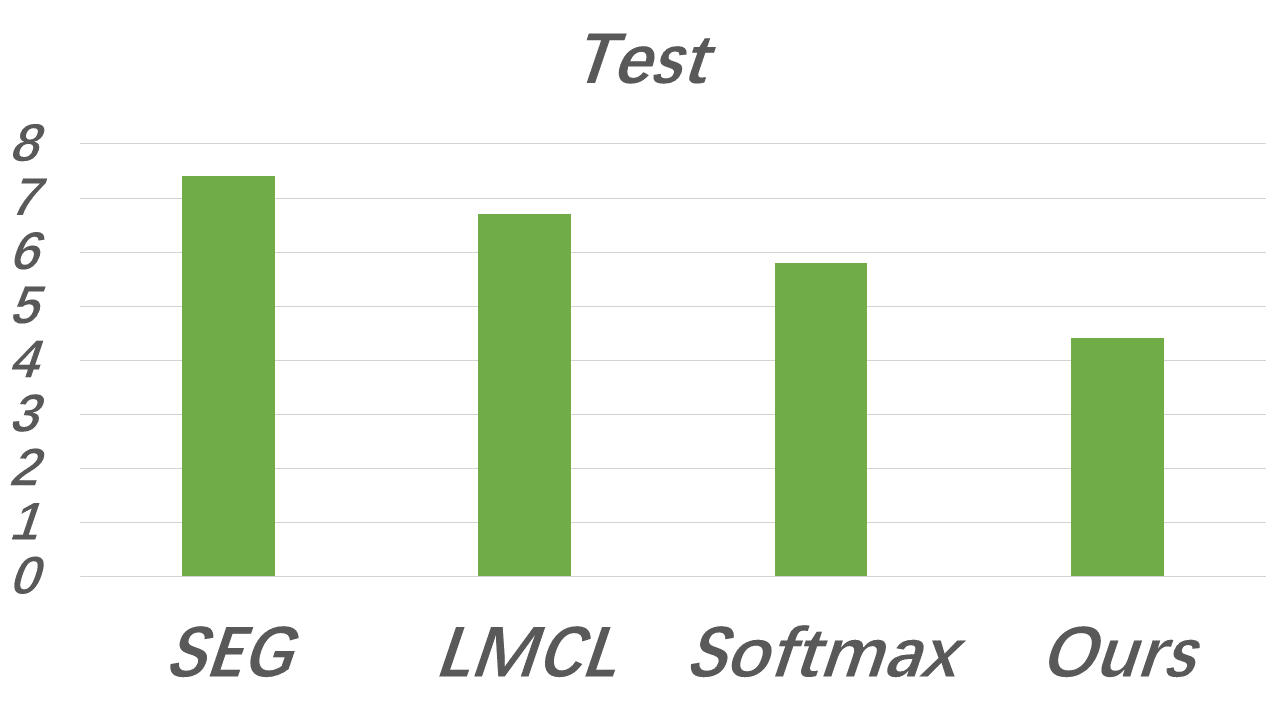
\includegraphics[width=1.\linewidth,height=0.11\textheight]{efficiency_test.png}
%   \caption{Self-Supervised Accuracy}
%   \label{fig:convex_acc}
\end{subfigure}%
\begin{subfigure}{0.23\textwidth}
  \centering
  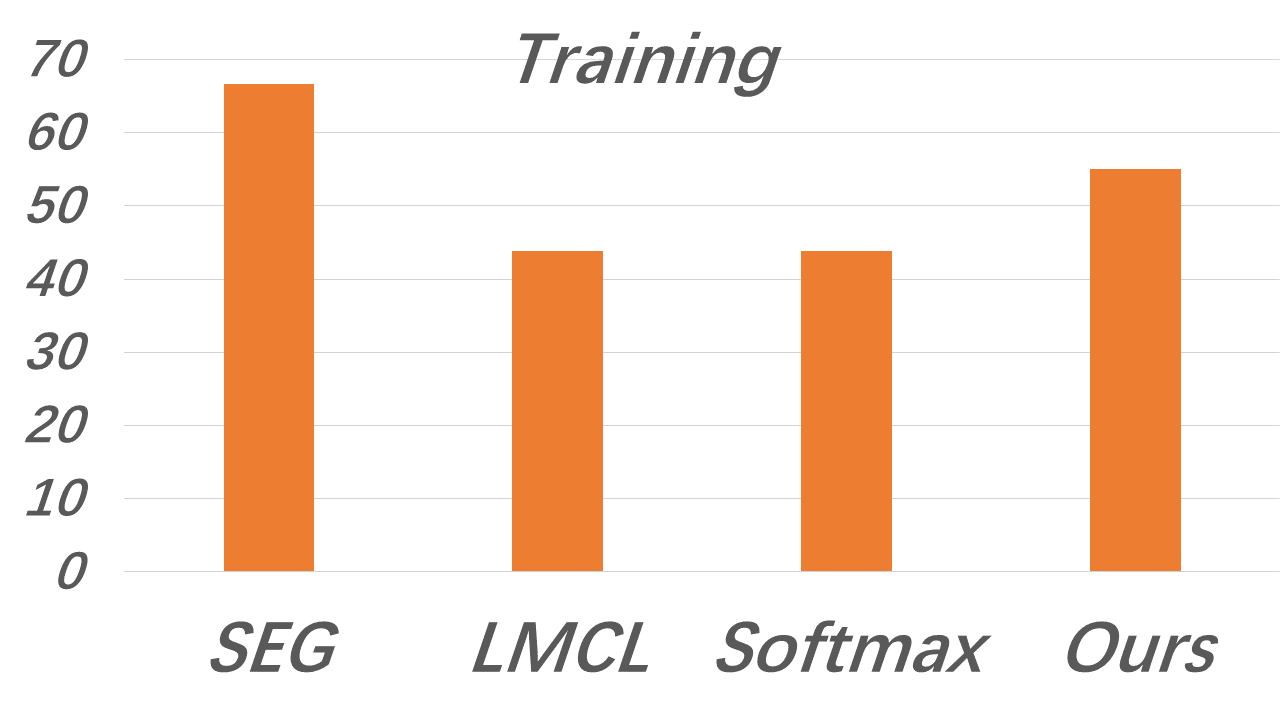
\includegraphics[width=1.\linewidth,height=0.11\textheight]{efficiency_train.png}
%   \caption{Self-Supervised Unknown F1}
%   \label{fig:convex_f1}
\end{subfigure}
\caption{Comparison of training time (per epoch) and test time with baselines.}
\label{fig:efficiency}
\end{figure}


\subsection{Efficiency}
We provide a quantitative comparison on the training and test efficiency for our method and the baselines, by calculating the average time (in seconds) for training per epoch and the total time for testing under the $75\%$ setting. Here, we only compare with the strongest baselines. As shown in Figure~\ref{fig:efficiency}, even with the pseudo outliers, the training time of our method is comparable to that of the baselines. Importantly, in the test stage, our method demonstrates significant advantages in efficiency, which needs much less time to predict intent classes for all samples in the test set.

% \begin{table}
% \centering
% % \setlength{\tabcolsep}{2.0pt}
% \small
% \begin{tabular}{lcccc}
% \hline
% Dataset&CLINK150&StackOverflow&Banking&MICD-EN\\
% \hline
% Vocab Size&8376&17,182&5028&1254\\
% \# Avg. Length&8.31&9.18&11.91&6.74\\
% \# of Samples&23,700&2,000&1,3083&1,745\\
% \hline
% \end{tabular}
% \caption{\label{table:datsets_stats}
% summary of datasets.
% }
% \end{table}

